\documentclass[
	fontsize=12pt,
	paper=a4,
	numbers=noenddot,
	listof=totoc,
	listof=entryprefix,
	listof=nochaptergap,
	bibliography=totoc,
	parskip=half,
	openany
]{scrbook}

\usepackage{cmap}


\usepackage[utf8]{inputenc}
\usepackage[T1]{fontenc}
\usepackage{lmodern}
\usepackage{ngerman}


\usepackage{scrhack}
\usepackage[table]{xcolor}
\usepackage{chngcntr}
\usepackage{enumitem}


\usepackage{amsthm}


\usepackage{lipsum}
\usepackage{unicode-math}


\usepackage{mathtools}


\usepackage[
	colorlinks=false,
	linkcolor=black,
	citecolor=black,
	filecolor=black,
	urlcolor=black,
	bookmarks=true,
	bookmarksopen=true,
	bookmarksopenlevel=3,
	bookmarksnumbered,
	plainpages=false,
	pdfpagelabels=true,
	hyperfootnotes
]{hyperref}


\renewcommand{\familydefault}{\sfdefault}
\usepackage[onehalfspacing]{setspace}
\raggedbottom

\usepackage{anyfontsize}

\addtokomafont{chapter}{\sffamily\large\bfseries}
\addtokomafont{section}{\sffamily\normalsize\bfseries}
\addtokomafont{subsection}{\sffamily\normalsize\mdseries}
\addtokomafont{caption}{\sffamily\normalsize\mdseries}

\usepackage{relsize}
\renewcommand*{\UrlFont}{\ttfamily\smaller\relax}


\usepackage[
	bindingoffset=0cm,
	inner=2.5cm,
	outer=2.5cm,
	top=3cm,
	bottom=2cm
]{geometry}

\usepackage[
	headsepline,
	plainheadsepline
]{scrlayer-scrpage}
\clearpairofpagestyles
\addtokomafont{pagehead}{\normalfont}
\ohead*{\thepage}
\ihead*{\leftmark}


\usepackage{graphicx}
\graphicspath{{pictures/}}
\usepackage{float}

\renewcommand{\thefigure}{\arabic{figure}}
\counterwithout{figure}{chapter}

\usepackage{wrapfig}


\usepackage{booktabs}
\usepackage{multirow}
\usepackage{tabularx}

\renewcommand{\thetable}{\arabic{table}}
\counterwithout{table}{chapter}


\usepackage{listings}
\usepackage{beramono}

\renewcommand{\lstlistlistingname}{List of Code Listings}
\renewcommand{\lstlistingname}{Code Listing}
\newcommand{\listoflolentryname}{\lstlistingname}

\definecolor{codegreen}{rgb}{0,0.6,0}
\definecolor{codegray}{rgb}{0.5,0.5,0.5}
\definecolor{codepurple}{rgb}{0.5,0,0.33}
\definecolor{codepurblue}{rgb}{0.16,0.0,1.0}
\definecolor{backcolour}{rgb}{0.95,0.95,0.92}

\lstdefinestyle{codestyle}{
	backgroundcolor=\color{backcolour},
	commentstyle=\color{codegreen},
	keywordstyle=\bfseries\color{codepurple},
	numberstyle=\tiny\color{codegray},
	stringstyle=\color{codepurblue},
	basicstyle=\scriptsize\ttfamily,
	breakatwhitespace=false,
	breaklines=true,
	captionpos=b,
	keepspaces=true,
	numbers=left,
	numbersep=5pt,
	showspaces=false,
	showstringspaces=false,
	showtabs=false,
	tabsize=2,
	escapeinside={(*@}{@*)}
}
\lstset{style=codestyle, numberbychapter=false}



\KOMAoptions{toc=chapterentrydotfill}
\addtokomafont{chapterentry}{\normalfont}
\setuptoc{toc}{totoc}

\DeclareTOCStyleEntry[beforeskip=0cm]{chapter}{chapter}
\DeclareTOCStyleEntry[beforeskip=0cm]{section}{section}
\DeclareTOCStyleEntry[beforeskip=0cm]{default}{subsection}

\BeforeStartingTOC[lof]{\def\autodot{:}}
\BeforeStartingTOC[lot]{\def\autodot{:}}
\BeforeStartingTOC[lol]{\def\autodot{:}}


\iffalse
\usepackage{csquotes}
\setlength\bibitemsep{.5\baselineskip}
\setcounter{biburlnumpenalty}{9000}
\setcounter{biburllcpenalty}{9000}
\setcounter{biburlucpenalty}{9000}

\fi

\usepackage[printonlyused]{acronym}


\usepackage[title,titletoc]{appendix}

\newcommand{\appendixchapter}[1]{
\cleardoublepage
\pagenumbering{arabic}
\renewcommand{\thepage}{\thechapter-\arabic{page}}
\chapter{#1}
}

\newcommand{\monthlyreport}[2]{
\section{#1}
\centering
\includegraphics[trim=55 35 55 35,clip,width=1\textwidth]{#2}
\clearpage
}



\newtheorem{beispiel}{Beispiel}

\newtheorem{these}{These}

\newtheorem{definition}{Definition}


\usepackage[nameinlink, noabbrev]{cleveref}


\lstset{
	extendedchars=true,
	inputencoding=utf8,
	literate=
		{ä}{{\"a}}1
		{ö}{{\"o}}1
		{ü}{{\"u}}1
		{ß}{{\ss}}1
		{Ä}{{\"A}}1
		{Ö}{{\"O}}1
		{Ü}{{\"U}}1
}

\begin{document}

\begin{titlepage}
	\pagestyle{empty}

	\begin{flushright}
		\begin{figure}[ht]
			\flushright
			
\includegraphics[height=2cm]{../../for_latex/hfu}
		\end{figure}
	\end{flushright}

	\begin{center}
		\vspace{3cm}

		{\fontsize{22}{22} \selectfont \textbf{Blatt 7}}\\[5mm]
		{\fontsize{18}{18} \selectfont Web-Security und Intrusion Prevention}

		\vspace{12cm}

		{\fontsize{14}{14} \selectfont Luis Staudt}
	\end{center}
\end{titlepage}


\chapter*{Aufgabe 1: Setup}

Keycloak wird über die bereitgestellte \texttt{docker-compose.yml} gestartet
(\texttt{docker compose up}). Die Compose-Datei mappt \verb|"8081:8080"|, sodass
die Admin-Konsole unter \url{http://localhost:8081} erreichbar ist
(containerintern Port 8080). Die Zugangsdaten werden über die Umgebungsvariablen
\texttt{KEYCLOAK\_ADMIN=admin} und \texttt{KEYCLOAK\_ADMIN\_PASSWORD=admin}
gesetzt; der Login erfolgt folglich mit \texttt{admin} / \texttt{admin} und damit
über ein Default-Passwort.

Die Admin-Konsole öffnet sich nach dem Login im Realm \emph{master}.

\chapter*{Aufgabe 2: User anlegen}

Im \emph{master}-Realm wird nur Keycloak selbst verwaltet. Für die Anwendung wird
daher ein eigener Realm \texttt{hfuBereich} angelegt und darin werden zwei
Benutzer erstellt:

\begin{itemize}
	\item \texttt{userCM}: Claudia Müller, \texttt{cm@hfuBereich.de}
	\item \texttt{userHM}: Hans Meier, \texttt{hm@hfuBereich.de}
\end{itemize}

\Cref{fig:kcusers} zeigt die Benutzerliste des Realms \texttt{hfuBereich} in der
Admin-Konsole mit beiden Benutzern.

\begin{figure}[H]
	\centering
	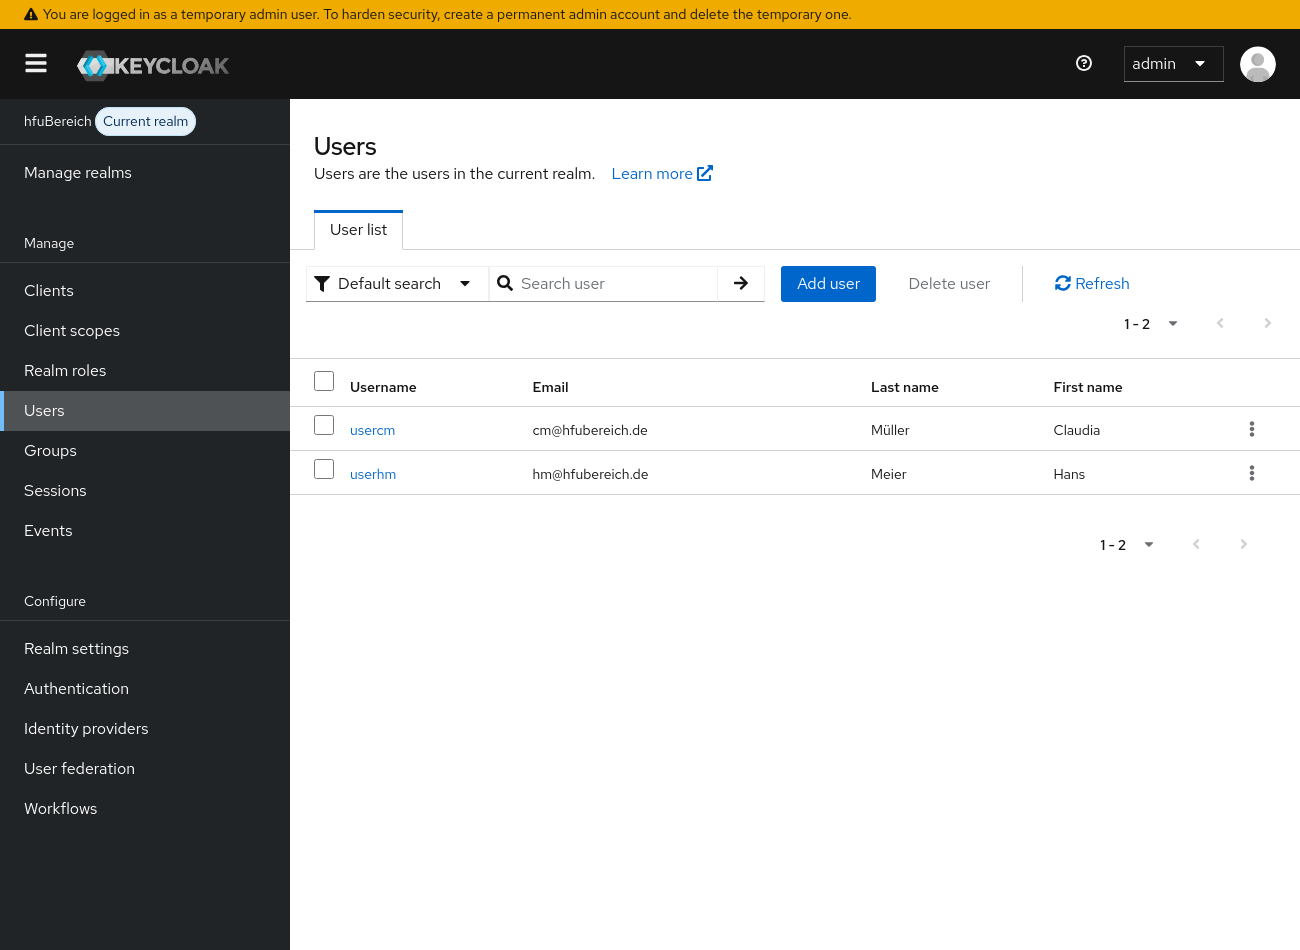
\includegraphics[width=\textwidth]{images/keycloak_users}
	\caption{Admin-Konsole, Realm hfuBereich, mit den Benutzern userCM und userHM.}
	\label{fig:kcusers}
\end{figure}

Für den Login-Test können sich die Benutzer über die Account-Konsole anmelden,
URL-Form \url{http://<Adresse>/realms/hfuBereich/account}. Damit der Login sofort
gelingt, muss den Benutzern ein nicht temporäres Passwort gesetzt werden, da
Keycloak andernfalls beim ersten Login einen Passwortwechsel erzwingt. Nach dem
Setzen eines Passworts (hier \texttt{test1234}) und \texttt{emailVerified=true}
gelingt die Anmeldung ohne weitere Schritte.

\chapter*{Aufgabe 3: MFA mit OTP konfigurieren}

Für \texttt{userHM} wird ein zweiter Faktor erzwungen, indem die Required Action
\texttt{CONFIGURE\_TOTP} gesetzt wird; alternativ lässt sich dies realmweit über
\emph{Authentication $\rightarrow$ Required Actions} konfigurieren.

Beim nächsten Login verlangt Keycloak die Einrichtung eines TOTP-Authenticators
(\emph{Mobile Authenticator Setup}) und zeigt einen QR-Code, der mit Google
Authenticator, FreeOTP oder vergleichbaren Anwendungen gescannt wird
(\Cref{fig:kcotp}). Anschliessend ist bei jeder Anmeldung zusätzlich zum Passwort
der sechsstellige Einmal-Code einzugeben; der zweite Faktor ist damit aktiv.

\begin{figure}[H]
	\centering
	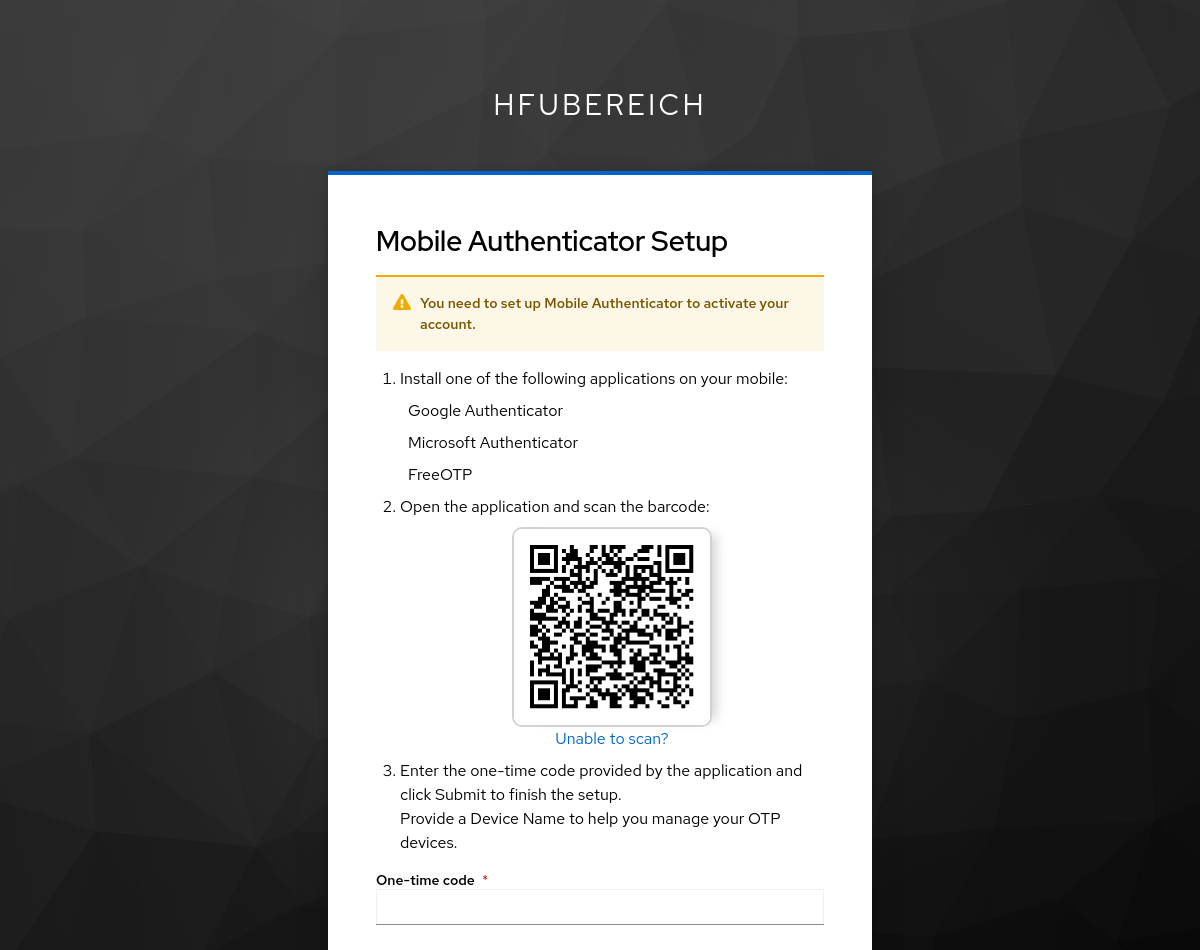
\includegraphics[width=0.6\textwidth]{images/keycloak_otp_setup}
	\caption{Erzwungene OTP-Einrichtung für userHM beim Login (QR-Code + Einmal-Code).}
	\label{fig:kcotp}
\end{figure}

\chapter*{Aufgabe 4: Service Provider (Nextcloud) per SAML anbinden}

Nextcloud soll als SAML-SP über Keycloak (IdP) angemeldet werden. Der Ablauf
gliedert sich in vier Schritte.

\textbf{1) IdP-Metadaten in Keycloak.} Unter \emph{Realm Settings} liefert
Keycloak die SAML-Metadaten des Realms. Die relevanten Werte sind:

\begin{lstlisting}[language=XML]
entityID (IdP) : http://<keycloak>/realms/hfuBereich
SSO-Endpoint   : http://<keycloak>/realms/hfuBereich/protocol/saml
Metadaten-URL  : http://<keycloak>/realms/hfuBereich/protocol/saml/descriptor
\end{lstlisting}

\textbf{2) SAML-Client in Keycloak.} Für Nextcloud wird ein Client vom Typ
\emph{saml} angelegt. Wichtige Einstellungen sind:

\begin{itemize}
	\item Client-ID = die SP-EntityID (Nextcloud-Metadaten-URL),
	      etwa \texttt{http://<nextcloud>/apps/user\_saml/saml/metadata}
	\item Valid Redirect URI / ACS:
	      \texttt{http://<nextcloud>/apps/user\_saml/saml/acs}
	\item \emph{Sign Assertions} aktiv, Name-ID-Format \texttt{username}
	\item Attribut-Mapper für \texttt{username}, \texttt{email},
	      \texttt{firstName} und \texttt{lastName}, damit Nextcloud die Felder
	      zuordnen kann.
\end{itemize}

\textbf{3) Nextcloud einrichten.} Die Nextcloud-Oberfläche wird geöffnet und ein
initialer Admin angelegt; die empfohlenen Apps, vor allem Nextcloud Office,
werden nicht installiert, da sie das Log fluten. Anschliessend wird die App
\emph{SSO \& SAML authentication} installiert und konfiguriert:

\begin{itemize}
	\item Attribut zur Identifikation des Nutzers: \texttt{username}
	\item IdP Entity ID, SSO-URL und das X.509-Signaturzertifikat des IdP aus den
	      Keycloak-Metadaten eintragen.
	\item Service-Provider-Daten (EntityID/ACS) passend zum Keycloak-Client.
\end{itemize}

\textbf{4) Funktionstest.} Beim Aufruf von
\url{/apps/user_saml/saml/login} wird der Browser zum Keycloak-Login (Realm
hfuBereich) weitergeleitet. Nach der Anmeldung als userCM leitet Keycloak mit
einer signierten SAML-Assertion (HTTP-POST-Binding) an den ACS-Endpunkt von
Nextcloud zurück, das daraufhin eine lokale Sitzung öffnet. \Cref{fig:ncsso}
zeigt das Ergebnis: userCM ist ohne separates Nextcloud-Passwort angemeldet, die
Attribute wurden korrekt übernommen (Full name \texttt{usercm}, E-Mail
\texttt{cm@hfubereich.de}).

\begin{figure}[H]
	\centering
	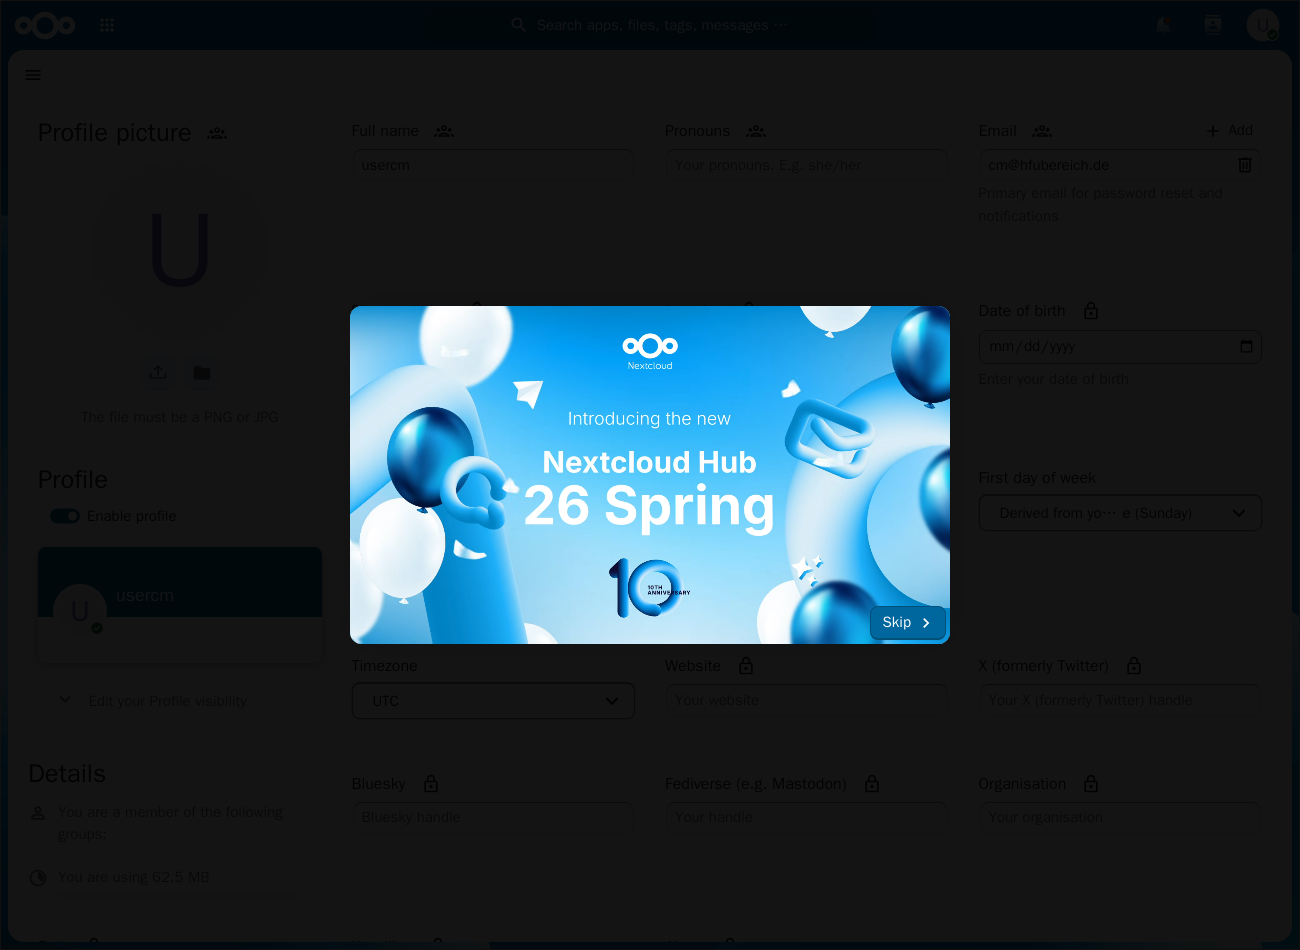
\includegraphics[width=\textwidth]{images/nextcloud_sso}
	\caption{Nextcloud nach SAML-SSO über Keycloak: userCM ist angemeldet, Attribute gemappt.}
	\label{fig:ncsso}
\end{figure}

Bei der Umsetzung waren zwei Punkte entscheidend:

\begin{itemize}
	\item \textbf{HTTPS ist Pflicht.} Die App \texttt{user\_saml} setzt ihr
	      Zustands-Cookie \texttt{saml\_data} mit \texttt{SameSite=None}. Moderne
	      Browser akzeptieren solche Cookies nur mit \texttt{Secure}-Flag, also
	      über HTTPS. Über reines HTTP ging das Cookie beim ACS verloren
	      (\glqq Cookie was not present\grqq{}), wodurch eine Redirect-Schleife
	      entstand. Als Lösung wurde Nextcloud hinter einen TLS-Reverse-Proxy
	      (NginX, selbstsigniertes Zertifikat) auf Port 8443 gestellt und
	      \texttt{overwritehost} sowie \texttt{overwriteprotocol} auf
	      \texttt{https} gesetzt.
	\item \textbf{Keine doppelten Attribute.} Der Default-Scope
	      \texttt{role\_list} erzeugt pro Rolle ein eigenes
	      \verb|<Attribute Name="Role">|. Nextcloud lehnt die Assertion dann mit
	      \glqq duplicated Name\grqq{} ab. Der Scope wurde daher vom Client
	      entfernt.
\end{itemize}

Das vollständige Setup (Keycloak-Konfiguration per Admin-REST-API, Nextcloud per
\texttt{occ}) liegt reproduzierbar als \texttt{setup-saml.sh} bei.

\chapter*{Vergleich: SAML-SSO}

Der IdP (Keycloak) übernimmt die Authentifizierung zentral; der SP (Nextcloud)
vertraut der signierten Assertion und führt selbst keine Passwortprüfung durch.
Wird ein zweiter Dienst an denselben IdP angebunden, entsteht Single-Sign-On:
Eine bestehende IdP-Sitzung wird wiederverwendet, sodass eine erneute Anmeldung
entfällt.


\end{document}
